%! TeX program = lualatex
\documentclass{book}

\usepackage[pl]{template}
% \usepackage[polish]{babel}

\title{Wrocławska Księga Matematyki}
\author{Weronika Jakimowicz}
\date{}

\makeatletter
\fancyfoot[CE, CO]{}
\fancyfoot[LE, RO]{\color{overlay2}\thepage}

\fancyhead[RE, LO]{$ \quad $\color{subtext1}Weronika Jakimowicz $ \quad $}
\fancyhead[LE, RO]{$ \quad $\color{green!40!subtext2}\bfseries \@title$ \quad $}


% \renewcommand{\chaptermark}[1]{\markboth{#1}{}}

\fancypagestyle{plain}{%
  \fancyhf{}%
  \fancyfoot[CE, CO]{}
  \fancyfoot[LE, RO]{\color{overlay2}\thepage}

  \fancyhead[RE, LO]{$ \quad $\color{subtext1}Weronika Jakimowicz $ \quad $}
  \fancyhead[LE, RO]{$ \quad $\color{green!40!subtext2}\bfseries \rightmark $ \quad $}
}
\makeatother

\begin{document}

\maketitle

\tableofcontents 

\chapter{Geometria Różniczkowa L2025}

\section{Przypadek krzywych}

\subsection{Krzywe na płaszczyźnie}

Jakościowo jesteśmy w stanie powiedzieć która z poniższych krzywych jest bardziej krzywa. 
\begin{center}
  
\begin{tikzpicture}
    \draw[thick] (0,0) to[out=0, in=-90] 
      (1, 1) to[out=90, in=-90] 
      (-1, 2) to[out=90, in=180] 
      (0, 3);
    \draw[thick] (2, 0) -- (2, 3);
  \end{tikzpicture}
\end{center}
Dodatkowo, lewa krzywa nie ma stałej krzywizny: są momenty gdzie zakręca, a są fragmenty gdzie jest niemalże prosta. Narzuca się pytanie, jak tę obserwację ująć w terminach matematycznych?

Zacznijmy od prostego przykładu, czyli okręgu na płaszczyźnie.
\begin{center}
  \begin{tikzpicture}
    \draw (0,0) circle (2);
    \draw (0,0) -- (30:2) node [midway, above] {$r$};

    \draw (4, 0) circle (1);
  \end{tikzpicture}
\end{center}
Okrąg w każdym punkcie ma taką samą krzywiznę, która dodatkowo maleje wraz ze wzrostem promienia okręgu.

\begin{definition}{krzywizna okręgu}{}
  Krzywiznę okręgu o promieniu $r$ definiujemy jako
  $$\kappa=\frac{1}{r}.$$
\end{definition}

Wróćmy jeszcze raz do pierwszego rysunku krzywych i wyobraźmy sobie okrąg styczny poruszający się po obu z nich z prędkością w punkcie będącą pochodną krzywej w tym punkcie. Na taki okrąg działa siła odśrodkowa, której będziemy używać do uogólnienia pojęcia krzywizny. 

Pojawia się jednak problem, gdyż wartość siły odśrodkowej dla tak podróżującego okręgu zależy nie tylko od tego jak bardzo krzywa jest krzywa, ale także od prędkości okręgu w wybranej parametryzacji krzywej. Będziemy więc chcieli ustandaryzować sposób, w jaki krzywe są nam prezentowane.

\begin{lemma}{o parametryzacji łukowej}{}
  Niech $\gamma:(a,b)\to\R^2$ będzie krzywą regularną, tzn. krzywą gładką o niezerowej pochodnej $\gamma'(t)\neq0$. Istnieje wówczas gładka reparametryzacja $s:(a,b)\to(0,l)$ taka, że $\gamma\circ s^{-1}$ jest krzywą o prędkości stale równej $1$. Innymi słowy,
  $$(\forall\;d\in (0,l))\;|(\gamma\circ s^{-1})'(d)|=1.$$
\end{lemma}

Powiemy, że krzywa jest \buff{sparametryzowana długością łuku}, jeśli ma pochodną stale równą $1$.

\begin{proof}TODO
  % Zdefiniujmy $s$ jako
  % $$s(t)=\in_a^t|\gamma'(u)|du.$$
  % Wtedy przeciwobraz krzywej $s$ w punkcie $u$ to droga, którą przebiliśmy od początku do teraz po krzywej $\gamma$.
\end{proof}

\begin{fact}{}{}
  Jeśli $\gamma$ jest sparametryzowana długością łuku, to $\gamma''(s)$ jest prostopadła do $\gamma'(s)$.
\end{fact}

\begin{proof}
  Długość wektora prędkości krzywej sparametryzowanej długością łuku jest stale równa jeden, czyli
  $$1=\langle \gamma'(s),\gamma'(s)\rangle$$
  dla każdego $s$. Możemy to wyrażenie zróżniczkować po $s$, otrzymując
  $$0=\frac{d}{ds}\langle \gamma'(s),\gamma'(s)\rangle=\langle \gamma''(s),\gamma'(s)\rangle+\langle \gamma'(s),\gamma''(s)\rangle=2\langle\gamma''(s), \gamma'(s)\rangle.$$
\end{proof}

\begin{definition}{znakowana krzywizna}{}
  Niech $\gamma$ będzie krzywą sparametryzowaną długością łuku. Niech $N(t)$ będzie wektorem jednostkowym takim, że $(\gamma'(t), N(t))$ jest ortogonalną, dodatnio zorientowaną bazą $\R^2$.
  \begin{center}
    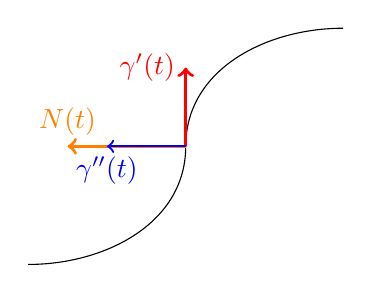
\begin{tikzpicture}
      \draw (-1,0) to[out=0, in=-90] (1, 1.5) to[out=90, in=180] (3, 3);
      \draw[red, very thick, ->] (1, 1.5) -- (1, 2.5) node[left] {$\gamma'(t)$};
      \draw[orange, very thick, ->] (1, 1.5)--(-.5, 1.5) node[above] {$N(t)$};
      \draw[blue, thick, ->] (1, 1.5)--(0, 1.5) node[below] {$\gamma''(t)$};
    \end{tikzpicture}
  \end{center}

  Wówczas \buff{znakowana krzywizna} $\kappa_\gamma(t)$ krzywej $\gamma$ w punkcie $t$ jest zdefiniowana równaniem
  $$\gamma''(t)=\kappa_\gamma(t)N(t).$$
\end{definition}

\begin{lemma}{(pierwsze) równania Freneta}{}
  Niech $\gamma$ będzie sparametryzowana długością łuku i niech $(T(s), N(s))$ będzie bazą ortonormalną dodatnio zorientowaną, gdzie $T(s)=\gamma(s)$. Wtedy
  $$T'=\kappa\cdot N$$
  $$N'=-\kappa T.$$
\end{lemma}

\begin{proof}TODO
\end{proof}

\begin{theorem}{podstawowe twierdzenie teorii krzywych}{podstawowe twierdzenie teorii krzywych 2d}
  Dla dowolnych 
  \begin{enumerate}
    \item $(x_0, y_0)\in\R^2$, 
    \item jednostkowego wektora $v\in \R^2$ 
    \item i gładkiej funkcji $\kappa:[0,b]\to\R$ 
  \end{enumerate}
  istnieje dokładnie jedna krzywa $\gamma:[0,b]\to\R^2$ sparametryzowana długością łuku zaczepiona w punkcie $(x_0, y_0)$ o początkowej prędkości $\gamma'(0)=v$ oraz krzywiźnie $\kappa_\gamma=\kappa$.
\end{theorem}

\begin{proof}TODO
\end{proof}

\begin{definition}{okrąg ściśle styczny}{}
  Niech $\gamma$ będzie krzywą sparametryzowaną długością łuku i niech $\eta$ będzie okręgiem sparametryzowanym długością łuku stycznym do $\gamma$ w punkcie $t$. Wtedy $\eta$ jest \buff{okręgiem ściśle stycznym} do $\gamma$, jeśli $\eta''(t)=\gamma''(t)$, tzn. jeśli mają tę samą krzywiznę.

  Możemy skonstruować nową krzywą, nazywaną \buff{ewolutą krzywej $\gamma$}, która składa się ze środków okręgów ściśle stycznych do $\gamma$:
  $$c=\gamma+\frac{1}{\kappa}N.$$
\end{definition}

Definicja okręgu ściśle stycznego w punktach samoprzecięcia krzywej $\gamma$ psuje się. Wtedy musimy zdecydować, czy chcemy takie punkty brać pod uwagę, czy zdefiniować okrąg ściśle styczny jako prostą. 

\begin{fact}{}{}
  Niech $\gamma$ będzie krzywą sparametryzowaną długością łuku taką, że $\kappa'(t)\neq0$. Wówczas okręgi ściśle styczne są parami rozłączne w otoczeniu punktu $t$.
\end{fact}

\begin{proof}TODO
\end{proof}

\subsection{Krzywe w przestrzeni}

Niech $\gamma:(a,b)\to \R^3$ będzie krzywą sparametryzowaną długością łuku taką, że $\gamma''(t)\neq 0$. Chcemy wybrać dodatnio zorientowaną, ortogonalną bazę $\R^3$, która będzie nieść ze sobą informacje o krzywej $\gamma$. Zdefiniujmy \buff{trójnóg Freneta} jako trójkę wektorów
\begin{itemize}
  \item $T(t)=\gamma'(t)$ to wektor styczny do krzywej,
  \item $N(t)=\frac{\gamma''(t)}{\|\gamma''(t)\|}$ jest znormalizowaną drugą pochodną $\gamma$,
  \item $B=T\times N$ jest nazywany wektorem binormalnym, czyli jednostkowym wektorem prostopadłym do płaszczyzny stycznej do $\gamma$.
\end{itemize}

\begin{definition}{torsja}{}
  \buff{Torsję $\tau$} krzywej $\gamma$ definiujemy jako wartość taką, że
  $$B'=-\tau N,$$
  gdzie $B$ i $N$ są wektorami jak wyżej.
\end{definition}

Wektory $T$ oraz $N$ rozpinają płaszczyznę, do której wektor $B$ jest prostopadły. Możemy ją zinterpretować jako płaszczyznę, na której zaczynamy rysować $\gamma$. Wtedy $\tau$ mówi jak szybko ołówek zaczyna uciekać z tej płaszczyzny.

\begin{theorem}{równania Ferneta}{}
  $$\frac{d}{dt}\begin{pmatrix}T&N&B\end{pmatrix} = \begin{pmatrix}T&N&B\end{pmatrix}\begin{pmatrix}
  0 & -\kappa & 0\\ 
  \kappa & 0 & -\tau\\ 
  0 & \tau & 0
\end{pmatrix}$$
\end{theorem}

\begin{proof}TODO
\end{proof}

\begin{theorem}{podstawowe twierdzenie teorii krzywych}{}
  Podobnie jak w twierdzeniu \ref{th:podstawowe twierdzenie teorii krzywych 2d}, chcemy pokazać, że dla ustalonych warunków początkowych, czyli 
  \begin{itemize}
    \item funkcji $\kappa:[0,b)\to\R_+$ krzywizny,
    \item funkcji $\tau:[0,b)\to \R$ torsji, 
    \item oraz dodatnio zorientowanej ortogonalnej bazy $(T,N,B)$ w $\R^3$
  \end{itemize}
  istnieje dokładnie jedna krzywa $\gamma:[0,b)\to\R^3$, której krzywizna i torsja to odpowiednio $\kappa$ i $\tau$, a trójnóg Ferneta w punkcie $t=0$ to $(T,N,B)$.
\end{theorem}

\begin{proof}TODO równania różniczkowe
\end{proof}

\subsection{Krzywizna powierzchni}

W tym rozdziale chcemy zdefiniować krzywiznę dla "ładnych" powierzchni w $\R^3$, tzn. powierzchni zadanych przez imersję
$$\Sigma:U\to \R^3$$
dla $U\subseteq\R^2$.

\begin{definition}{metryka Riemanna}{}
  Dla dowolnego punktu $p\in U\subseteq\R^2$ definiujemy dodatnio określoną dwuliniową formę $\langle-,-\rangle_\Sigma$, która dla wektorów stycznych $v_p,w_p\in T_pU$ przyjmuje wartość
  $$\langle v_p, w_p\rangle_\Sigma=\langle d\Sigma(v_p), d\Sigma(w_p)\rangle.$$
  Funkcja, która każdemu $p\in U$ przypisuje formę $\langle-,-\rangle_\Sigma$ na $T_pU$ nazywamy \buff{metryką Riemanna} na $U$.
\end{definition}

Dla wygody będziemy oznaczać
$$\partial_x=d\Sigma(\partial_x)$$
$$\partial_y=d\Sigma(\partial_y)$$
jako popchnięcie standardowego pola wektorowego na $\R^2$ przez $\Sigma$.

\begin{definition}{wektor normalny}{}
  Wektor normalny do powierzchni $\Sigma$ w punkcie $p$ to 
  $$n_p=\frac{\partial_x\times\partial_y}{\|\partial_x\times\partial_y\|}$$.
\end{definition}

W dowolnym punkcie powierzchni, przestrzeń do niego styczna jest dwuwymiarowa. Wybranie pojedynczego wektora stycznego tak jak w przypadku krzywych jest więc niemożliwe. Możemy za to zdefiniować krzywiznę powierzchnie w punkcie jako funkcję
$$\kappa:S^1\to\R.$$

\begin{definition}{}{}
  Dla $v\in T_p\Sigma$ długości $1$ definiujemy \buff{krzywiznę} w punkcie $p$ wzdłuż $v$, $\kappa_p(v)$, jako krzywiznę krzywej planarnej będącej przecięciem $\Sigma$ z płaszczyzną rozpiętą przez $v$ oraz $n_p$.
  \begin{center}
    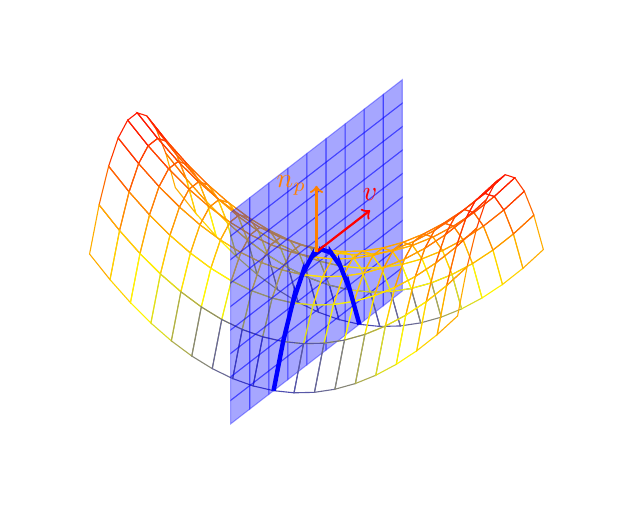
\begin{tikzpicture}\pgfplotsset{set layers}
      \begin{axis}[axis on top=false, samples=10, axis line style={draw=none}, yticklabel=\empty, xticklabel=\empty, zticklabel=\empty, tick style={draw=none}]
          \addplot3[mesh, y domain=-2:2, domain=-2:0] {x^2-y^2};
          \addplot3 [
            surf,
            domain=-4:4,
            opacity=0.35,
            fill=blue,
            draw=blue,
            colormap={solidblue}{color=(blue) color=(blue)},
            shader=flat
            ] ({0},{y},{x}); 
          \addplot3[mesh, domain=0:2, y domain=-2:2] {x^2-y^2};
          \addplot3[domain=-0.01:0.01, y domain=-2:2, ultra thick, blue] (0,{y},{x^2-y^2});

          \addplot3[
            ->,
            thick,
            red
          ]
          coordinates {(0,0,0) (0,2.5,0)}
          node [pos=1, above] {$ v$};
          
          \addplot3[
            ->,
            thick,
            orange 
          ]
          coordinates {(0,0,0) (0,0,2.5)}
          node[pos=1, left] { $n_p$ };
       \end{axis}
    \end{tikzpicture}
  \end{center}
\end{definition}


 
\end{document}
